\chapter{Testing and Evaluation}
\label{chap:testing}
This chapter assesses the proposed system's performance under a realistic load, complete with attack scenarios. The goal is to evaluate the trade-offs between availability, resilience and latency, under a directed volumetric attack. The target we are using is a NodeMCU development board, with an ESP8266 microcontroller SoC, running an HTTP microservice.

\section{Evaluation Metrics}
The effectiveness of the proposed solution is measured using multiple metrics. Each of these metrics play a different role in determining how viable our solution would be in a real world scenario, from the point of view of the client and the infrastructure.

\subsection{Delay times}
Delay times, or in short, latency, is crucial to the user experience and is measured in both favorable, nominal and stressful conditions. This is what the client experiences when he uses the service under our current system. From his point of view, the increased latency shouldn't be more than what the average service can be accessed, otherwise the user may choose to abandon the service.

In the tests which we conducted we used the timing statistics generated by the built-in function of Locust library from Python.

\subsection{Failure rate}
Beyond raw loading times, another very important metric is the failure rate. Considering our architecture and algorithm, the failure rate presents itself as a problem inherent to our solution only in the case of a DDoS attack. Simply by implementing an IP renewal strategy, the failure rate is not going to be perfect for the legitimate clients. These tests are also measured using the Locust and Requests libraries. 


\subsection{Power usage}
Given that most IoT devices are operated in environments with limited power sources, energy efficiency serves a dual purpose - it indicates how much time the IoT device can function, given a limited power supply, such as a battery, and also the performance at which it can run, since this is also tied to the limited power supply problem. Simply by using the system more, the application running on the OS will consume more power, when queried by a client.

The power usage is measured using a laboratory bench power supply-the development board has its power rail tied to the output of the power supply unit (PSU). The PSU can measure the power draw with a 1Hz refresh rate, and can export the statistics to the PC. After exporting the relevant data, a Matlab script was used to compile the results into \autoref{fig:power-usage}. The refresh rate of the PSU is not an impediment, as an average of the power consumption being measured once per second is adequate for capturing macro-level behavior and longer-term trends. While it may not reflect very short spikes in consumption at a millisecond level, the measurement resolution is sufficient for observing the effects of sustained traffic, similar to those caused by a volumetric flood.

\section{Simulation Environment}
The testbed used for evaluation simulates a microservice-based IoT system using a NodeMCU development board, with an ESP8266 microcontroller SoC. The clients are simulated through docker containers, the critical infrastructure is composed of different VMs, and the botnet is simulated both by using the Locust library and with an Ixia Breakingpoint packet generator appliance, capped at 1Gbps traffic.

Four traffic scenarios were considered:

\begin{itemize}
    \setlength\itemsep{1pt}
    \setlength\topsep{1pt}
    \setlength\parsep{1pt}
    \setlength\parskip{1pt}
    \item A baseline, idle system with no active clients, to establish reference power consumption and responsiveness.
    \item A normal usage pattern, with up to 10 requests per second, to represent a functioning system in typical operation.
    \item A DDoS using the Locust framework on the IoT device, during which the system is not active, to establish a comparison baseline.
    \item A final DDoS scenario using volumetric traffic from simulated clients, mimicking the behavior of a large-scale botnet attempting to overwhelm the service.
\end{itemize}

\section{Simulation Benchmark}
In this section we explain the results of our testing.

In nominal usage of the microservice, we extracted the following statistics from \autoref{fig:nominal-statistics}\cite{vladescu2025}. The requests per second (RPS) metric is between 3 and 4, even though the total number of users equates to 10. What is observable is that even without a high number of users, there still are failures, which is surprising, given the low number of clients. This shows how vulnerable are IoT devices of this kind to a volumetric DDoS. 

\begin{figure}
    \centering
    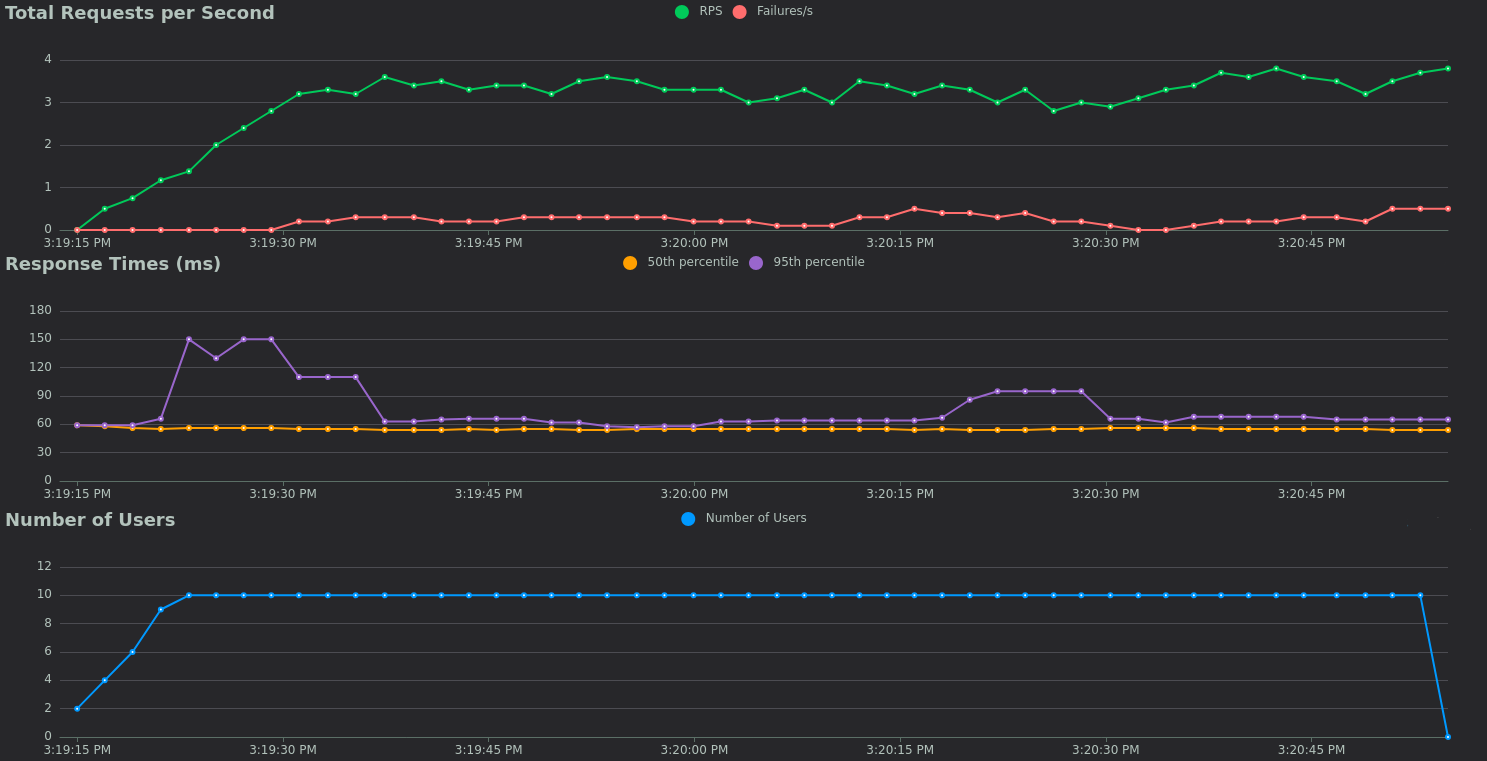
\includegraphics[width=0.8\linewidth]{images/nominal_usage.png}
    \caption{Locust Nominal Statistics}
    \label{fig:nominal-statistics}
\end{figure}

A response time of around 60ms is observed as a median, and as an extreme is peaking up to 150ms. This is acceptable, 150ms is not a big delay for an HTTP request, as most websites load in more time than the peak of this device.

As a big contrast, \autoref{fig:ddos-statistics}\cite{vladescu2025} shows a different statistic, in the case of an unprotected DDoS. The maximum user base is limited to 10,000, with users ramping with a rate of 100/s. The users will experience a big delay, which Locust does not record more than 20s, but this practically shows that the IoT microservice is almost instantly flooded, as the request per second curve matches, albeit in a delay, the failure per second curve.

\begin{figure}
    \centering
    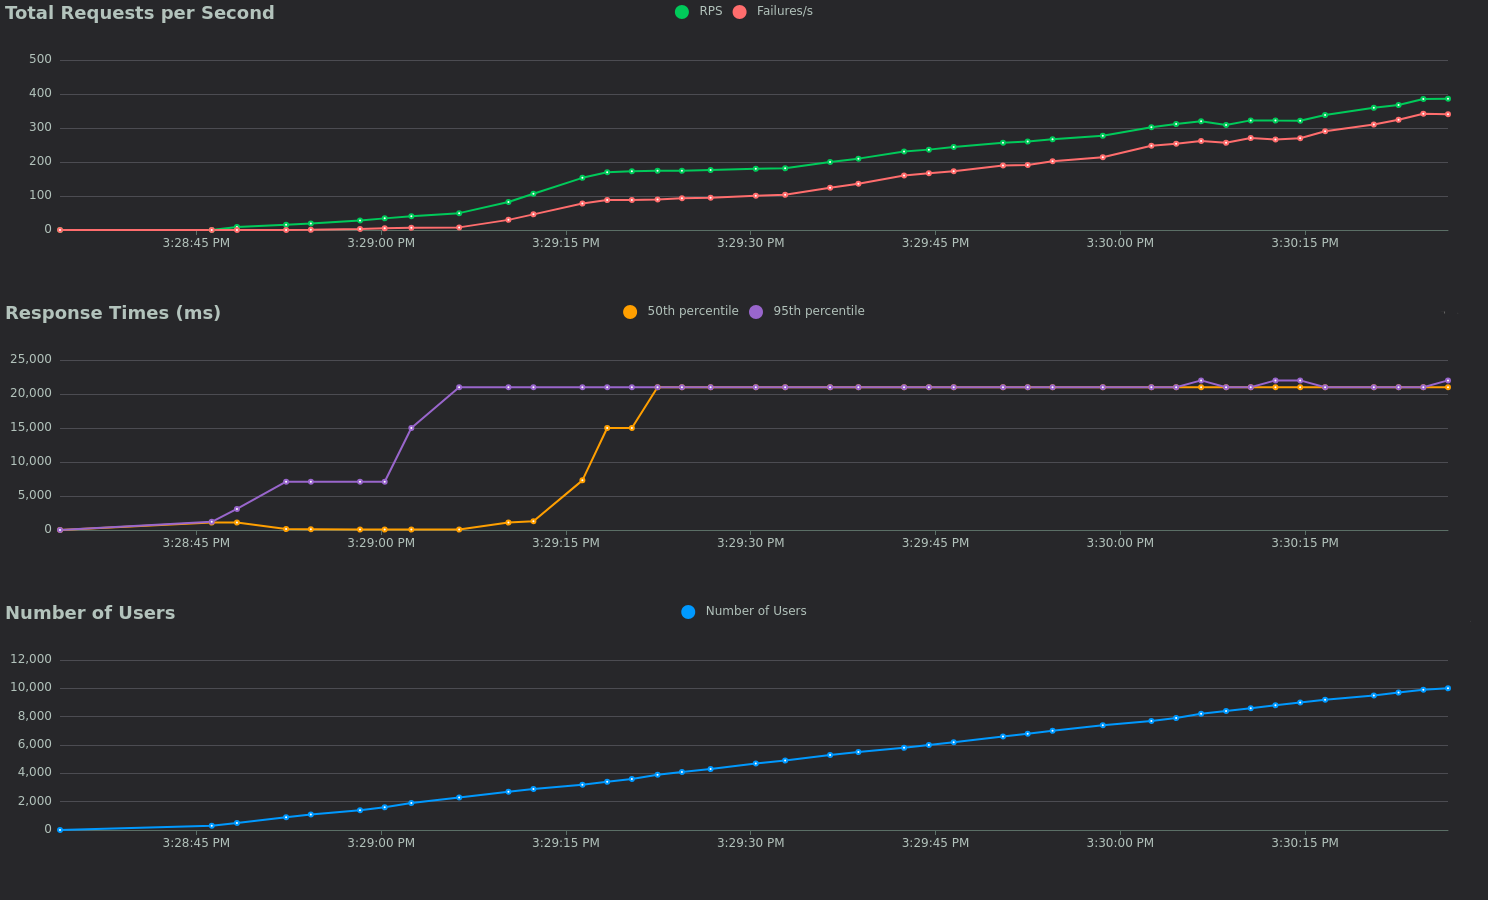
\includegraphics[width=0.8\linewidth]{images/ddos_usage.png}
    \caption{Locust Unprotected DDoS Statistics}
    \label{fig:ddos-statistics}
\end{figure}

To test how our system behaves with the security measures active and in-place, we used the Ixia Breakingpoint, with the specific data rate curve expressed in \autoref{fig:data-rate}\cite{vladescu2025}. This assures that the attackers are generated in a truly realistic scenario, without having software components to throttle the system-the Ixia packet generator can easily generate 1Gbps traffic of HTTP requests. To find just how vulnerable the IoT microservice is, we can consult \autoref{fig:power-usage}\cite{vladescu2025}, where we can see curves of power usage for each of the cases tested. 

We can see with green a baseline without clients, where the power draw averages a value almost constant to 3.9 Watts. With blue we can differentiate how clients consume data from the IoT server, since the power usage spikes reach up to 4 Watts. 

\begin{figure}
    \centering
    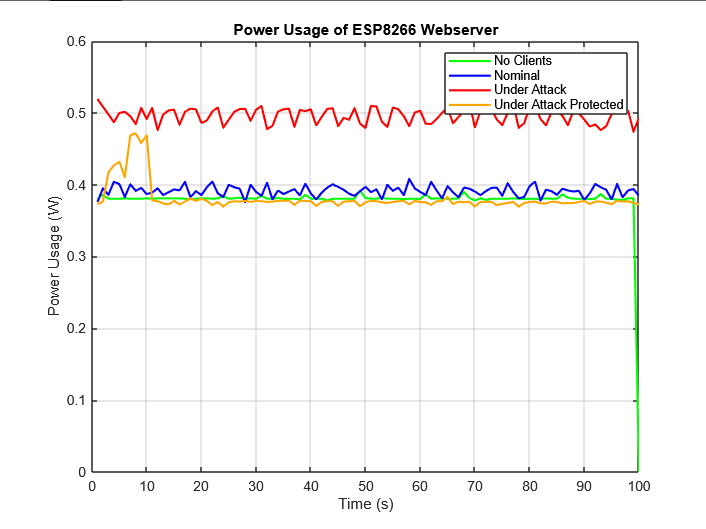
\includegraphics[width=0.8\linewidth]{images/power_usage_esp8266.png}
    \caption{Power Usage of ESP8266 Webserver in Different Scenarios}
    \label{fig:power-usage}
\end{figure}

In the realistic DDoS scenario, we can see the red curve, with jumps above the 5 Watt marker, thus consuming more than 165\% power compared to the nominal load. This equates to diminishing the IoT's battery from a nominal usage of one year to about seven months, time in which it isn't available due to the high traffic. This study doesn't take into consideration the dangers of overloading an SoC, but there are certainly problems stemming from continous usage, with an increased temperature footprint. The last green sample is not to be taken into consideration, as it represents a mismatch in data length, not an outlier of data.

When the system protection is activated, the power curve is similar to the one colored with orange. The power usage is slightly shifted, since the green would overlap the orange, we believe this anomaly is due to a measurement error in the decimals of the laboratory power supply combined with other external factors, such as temperature or transient currents. There is a big spike observed in the first 10 seconds, where the system blocks most of the offending hosts, and the IoT can serve legitimate clients.

